\documentclass[a4paper,12pt,oneside]{book}
\usepackage[utf8]{inputenc}
\usepackage[T1]{polski}
\usepackage{helvet}
\usepackage{graphicx}
\usepackage{color}
\usepackage{geometry}
\usepackage{fancyhdr}

\fancyfoot[C]{\thepage}
\pagestyle{plain}
\geometry{hmargin={2cm, 2cm}, height=10.0in}
\usepackage{float}
\usepackage{url}
\usepackage[colorlinks=false, pdfborder={0 0 0}]{hyperref}

\title{Symulacja komputerowa zaniku sygnału luminescencyjnego w skaleniach}
\author{Olaf Schab}

\begin{document}
\thispagestyle{empty}

\includegraphics[height=37.5mm]{agh_nzw_a_pl_1w_wbr_cmyk.eps}\\
\rule{30mm}{0pt}
{\large\textsf{Wydział Fizyki i Informatyki Stosowanej}}\\
\rule{\textwidth}{3pt}\\
\rule[2ex]
{\textwidth}{1pt}\\
\vspace{7ex}
\begin{center}
{\bf\LARGE\textsf{Praca inżynierska}}\\
\vspace{13ex}
% --------------------------- IMIE I NAZWISKO -------------------------------
{\bf\Large\textsf{Olaf Schab}}\\
\vspace{3ex}
{\sf \small kierunek studiów:} {\bf\small\textsf{informatyka stosowana}}\\
\vspace{15ex}
%% ------------------------ TYTUL PRACY --------------------------------------
{\bf\huge\textsf{Symulacja komputerowa zaniku sygnału luminescencyjnego w skaleniach}}\\
\vspace{14ex}
%% ------------------------ OPIEKUN PRACY ------------------------------------
{\sf \Large Opiekun:} {\bf\Large\textsf{dr inż. Grzegorz Gach}}\\
\vspace{22ex}
\textsf{\bf\large\textsf{Kraków, styczeń 2017}}
\end{center}
%% =====  STRONA TYTUŁOWA PRACY INŻYNIERSKIEJ  ====

\newpage

%% =====  TYŁ STRONY TYTUŁOWEJ PRACY INŻYNIERSKIEJ  ====
{\sf Oświadczam, świadomy(-a) odpowiedzialności karnej za poświadczenie nieprawdy, że niniejszą pracę dyplomową wykonałem(-am) osobiście i samodzielnie i nie korzystałem(-am) ze źródeł innych niż wymienione w pracy.}

\vspace{14ex}

\begin{center}
\begin{tabular}{lr}
~~~~~~~~~~~~~~~~~~~~~~~~~~~~~~~~~~~~~~~~~~~~~~~~~~~~~~~~~~~~~~~~~ &
................................................................. \\
~ & {\sf (czytelny podpis)} \\
\end{tabular}
\end{center}

\newpage
\linespread{1.3}
\selectfont
\newpage
\textbf{Merytoryczna ocena pracy przez opiekuna}
\newpage
\textbf{Merytoryczna ocena pracy przez recenzenta}
\noindent


\vspace{85mm}
\tableofcontents


\chapter{Wstęp}
Do określenia wieku próbek w archeologii i geologii wykorzystywane są skalenie z uwzględnieniem stymulowanej luminescencji. Już w latach 60- tych  XX wieku powstał pomysł wykorzystania termoluminescencji, która dzięki badaniom znalazła wiele zastosowań w archeologii i naukach o Ziemi. Jednym z głównych tematów badań jest datowanie z wykorzystaniem skaleni przy użyciu ich termoluminescencji oraz atermicznym zanikiem luminescencji powodującym zaniżanie daty próbek. Atermiczny zanik związany jest z faktem zachodzenia rekombinacji zlokalizowanej, głownie poprzez zachodzące zjawisko tunelowania elektronów z pułapek elektronowych oraz centrów rekombinacyjnych. 

\section{Założenia projektu}
Celem projektu było stworzenie programu symulującego zanik sygnału luminescencyjnego w skaleniach. Głównym założeniem było otrzymanie wykresu obrazującego zmianę ilości elektronów znajdujących się w stanie wzbudzonym (znajdujących się w pułapkach) wraz z upływem czasu.

\section{Zjawisko luminescencji w skaleniach}


Jednym ze składników środowiska naturalnego jest promieniowanie jonizujące. Najważniejszym jego źródłem są izotopy promieniotwórcze zawarte w skorupie ziemskiej, atmosferze
i biosferze, emitujące promieniowanie $\alpha$, $\beta$ i $\gamma$. 
W ostatnim okresie, bardzo krótkim w sensie geologicznym oraz historycznym, pojawiły
się nowe jego źródła, związane z działalnością człowieka w zakresie zbrojeń atomowych
i energetyki jądrowej. W dalszym jednak ciągu najważniejszym źródłem promieniowania
jonizującego w środowisku są izotopy promieniotwórcze, które weszły w skład Ziemi w okresie
formowania się układu słonecznego.  Są to przede wszystkim długożyciowe izotopy uranu $U^{238}$, $U^{235}$ i toru $Th^{232}$. Promieniowanie to niesie energię, którą pochłaniają wszystkie substancje występujące
w środowisku - w tym skalenie. I to właśnie pochłanianie promieniowania jonizującego przez te kryształy jest związane z luminescencją.

Rzeczywisty kryształ nie jest idealny. Zawiera on zawsze nieregularności i defekty struktury sieci krystalicznej. Część z nich znajdująca się w paśmie wzbronionym może mieć charakter pułapek, które są zdolne do wychwytywania
elektronów z pasma przewodnictwa i przetrzymywania ich przez długi czas, do
momentu, w którym otrzymają one energię niezbędną do wzbudzenia do pasma przewodnictwa. Stan kryształu, w którym część lub wszystkie pułapki są zapełnione schwytanymi elektronami,
charakteryzuje się nadwyżką energii w porównaniu ze stanem podstawowym.  Nadwyżka ta może zostać wyzwolona i wyemitowana np. w postaci światła poprzez dostarczenie dodatkowej energii (podgrzanie kryształu lub jego oświetlenie). Właśnie to zjawisko wykorzystywane jest w metodach datowania obiektów archeologicznych
i osadów geologicznych do pomiarów dawek pochłoniętych naturalnego
promieniowania jonizującego 
\begin{figure}[h]
\centering
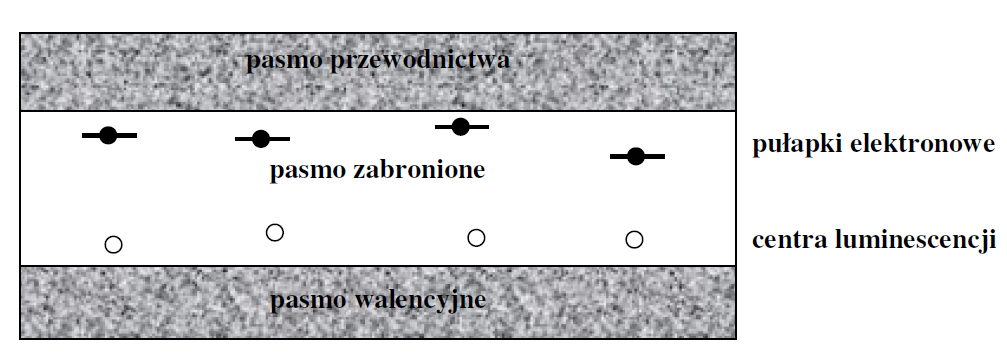
\includegraphics[width=15cm]{strukturapasmowa}
\caption{Struktura pasmowa skalenia.}
\label{fig:Struktura pasmowa}
\end{figure}

Zdarza się jednak, że mimo iż uwięziony elektron nie otrzymał dodatkowej energii, będzie w stanie zrekombinować z dziurą. Jest to jest możliwe dzięki  \textbf{zjawisku tunelowania}.

\section{Zjawisko tunelowania (Zjawisko emisji polowej)}
Zjawisko emisji polowej, zwane tunelowaniem Fowlera – Nordeheima, to  proces kwantowo-mechaniczny w którym cząstka ma niezerowe prawdopodobieństwo przejścia przez barierę potencjalną nawet, gdy energia cząstki jest mniejsza od wysokości bariery potencjału.


\begin{figure}[H]
\centering
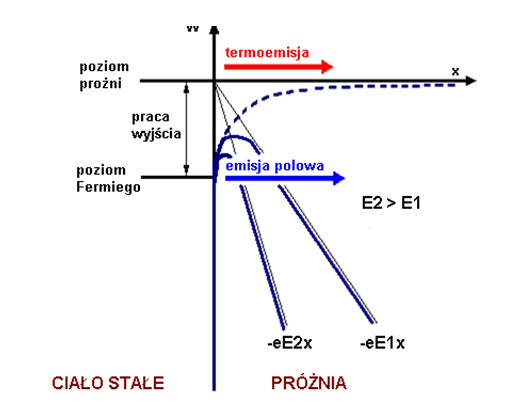
\includegraphics[width=10cm]{tunelowanie}
\caption{Ilustracja mechanizmu emisji polowej.}
\label{fig:Tunelowanie}
\end{figure}



Analizując powyższy wykres można stwierdzić, że im wyższa wartość przyłożonego zewnętrznego pola tym węższa staje się bariera potencjału, a prawdopodobieństwo tunelowania wzrasta. 

W przypadku skaleni prawdopodobieństwo, że elektron nie przetuneluje do centrum rekombinacji wyrażone jest wzorem:

\begin{equation}
\label{eq:1}
P = e^{\frac{-t}{\tau}}
\end{equation}

\begin{equation}
\tau = S^{-1}e^{\alpha r}
\end{equation}


gdzie:
\begin{itemize}
\item t - czas
\item S - stała częstotliwość prób ucieczki
\item $\alpha$ -  stała zależna od różnicy energii pułapki i dziury
\item r - odległość do przetunelowania
\end{itemize}







\chapter{Wybór stosowanych technologii}
\section{Język C++11 oraz wybór kompilatora}
Aplikacja została napisana z użyciem języka C++11 \cite{c++}. Język ten
wybrano z kilku powodów. Skorzystano tu z jego natury jako języka zorientowanego obiektowo. Dzięki temu podczas wykonania programu stworzono klasy odpowiadające obiektom w świecie realnym - elektrony, pułapki elektronowe itp.
Kolejnym powodem dla którego wykorzystano język C++ jest jego wydajność. Kod napisany
w języku C++ jest kompilowany bezpośrednio i w pełni do kodu maszynowego  wykonywanego przez procesor komputera. Dzięki temu
otrzymujemy maksymalną możliwą wydajność inaczej niż gdy używamy innych
obiektowych języków programowania wysokiego poziomu, które są kompilowane do kodu
zarządzanego (tzw. kodu bajtowego na przykład w przypadku Javy) gdzie dodatkowy narzut
generowany jest przez warstwę pośrednią w postaci maszyny wirtualnej. 

C++11 jest standardem języka C++ zastępującym standard C++03. Wprowadza on kilka dodatków do rdzenia języka oraz znacznie rozszerza bibliotekę standardową C++. Dla przykładu wprowadza on słowo kluczowe \textit{auto} jako zastępczy typ zmiennej, który zostanie wydedukowany na podstawie wartości za pomocą której zmienna zostanie zainicjalizowana. Nowa biblioteka wprowadza również kilka silników do generacji liczb pseudolosowych. W projekcie wykorzystano generator oparty na jednostajnie ciągłym rozkładzie prawdopodobieństwa.

Do kompilacji użyto darmowego kompilatora GCC (Gnu Compiler Collecion), konkretnie jego implementacji dla platformy Windows - MinGW w wersji 3.2.2 (Minimalist GNU for Windows).

\section{Środowisko programistyczne}

Program był tworzony z użyciem wieloplatformowego zintegrowanego środowiska programistycznego języków C/C++ - \textbf{CLion} (wersja 2016.2.3) produkcji spółki JetBrains. Było to podyktowane głównie znajomością produktów firmy JetBrains. \href{https://www.jetbrains.com/clion/}{CLion} jest produktem komercyjnym, jednak skorzystano tu z darmowej licencji studenckiej. IDE produkcji JetBrains obsługuje również 	system zarządzania kompilacją \textbf{CMake}, którego główną cechą jest niezależność od używanego kompilatora oraz platformy sprzętowej - CMake nie kompiluje programu samodzielnie, lecz tworzy pliki z regułami kompilacji dla konkretnego środowiska.

\begin{figure}[h]
\centering
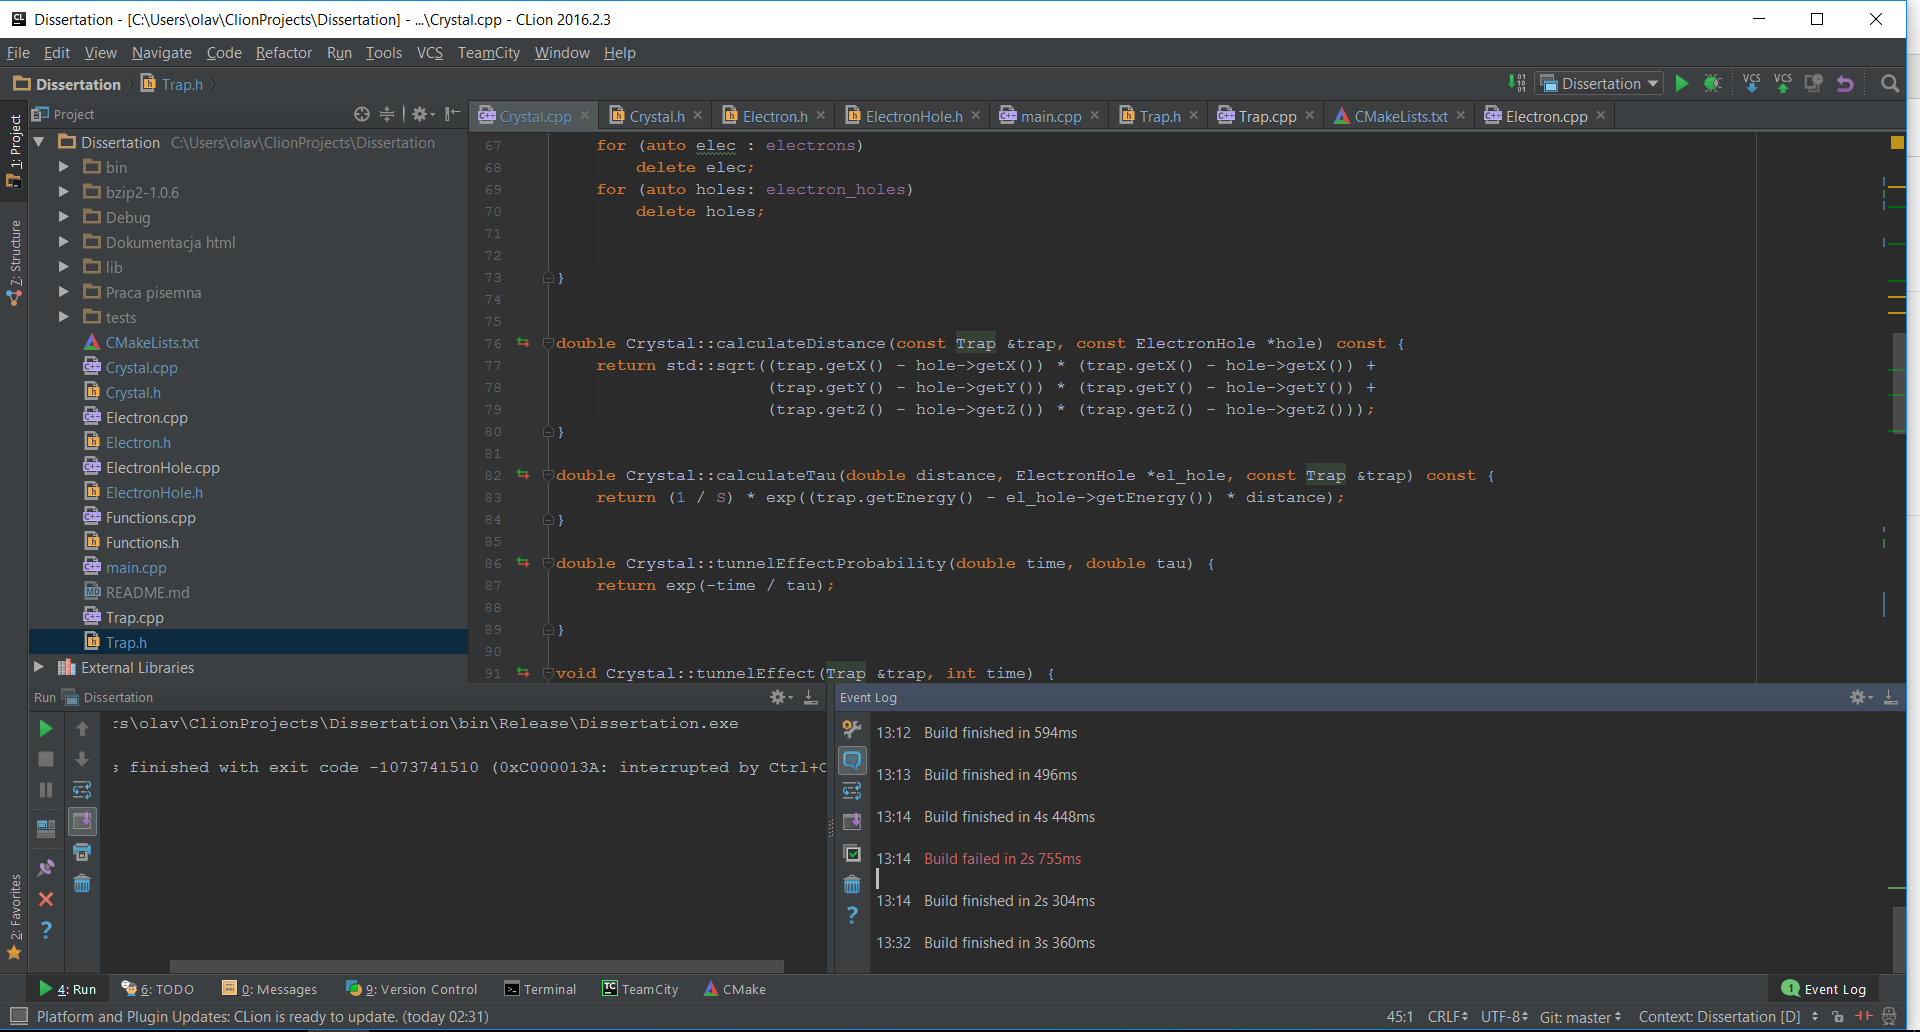
\includegraphics[width=17cm]{clion}
\caption{Wygląd okna programu CLion \cite{struktura_pasmowa}}
\label{fig:clion}
\end{figure}

Dużą zaletą podczas pracy z IDE produkcji JetBrains jest jego intuicyjna i prosta obsługa całości projektu. Dodatkowo, CLion posiada możliwość bezpośredniego połączenia projektu z wybranym serwerem kontroli wersji co uprościło pracę nad projektem. Z racji tego, że w chwili obecnej program do kompilacji używa tylko systemu CMake, niezbędne było nauczenie się jego obsługi  oraz odpowiedniej składni.
Ostatecznie kod pliku \emph{CMakeLists.txt} wygląda następująco:
\begin{verbatim}

cmake_minimum_required(VERSION 3.6)
project(Dissertation)
set(CMAKE_EXE_LINKER_FLAGS "-static-libgcc -static-libstdc++ -static")
set(CMAKE_CXX_FLAGS "${CMAKE_CXX_FLAGS} -std=gnu++11 -O2 -g -Wall")
SET(CMAKE_FIND_LIBRARY_SUFFIXES ".a")
SET(BUILD_SHARED_LIBRARIES OFF)
set(SOURCE_FILES main.cpp Electron.h Electron.cpp Trap.cpp Trap.h Functions.cpp Functions.h ElectronHole.cpp ElectronHole.h Crystal.cpp Crystal.h)
add_executable(Dissertation ${SOURCE_FILES})
target_link_libraries(Dissertation)

\end{verbatim}
\section{System kontroli wersji Git}

System kontroli wersji śledzi wszystkie zmiany dokonywane w plikach i umożliwia przywołanie dowolnej wcześniejszej wersji. Jest to przydatne narzędzie w łączeniu zmian dokonanych przez wiele osób w różnym czasie.

W procesie tworzenia aplikacji wykorzystano system kontroli wersji Git oraz darmowy hostingowy serwis internetowy \href{https://github.com/}{GitHub}.
Głównym powodem wykorzystania tego systemu była jego popularność oraz prostota użytkowania.
System kontroli wersji okazał się być niezwykle użytecznym narzędziem pozwalającym na
śledzenie zmian w kodzie, wprowadzanie testowych rozwiązań bez
ryzyka zniszczenia kodu. Cały projekt można pobrać ze strony:
\begin{center}
\url{https://github.com/Sharkuu/Dissertation}
\end{center}

\section{Wizualizacja wyników - Gnuplot}

Po wygenerowaniu danych, aby z wizualizować wykres obrazujący zmianę ilości elektronów znajdujących się w stanie wzbudzonym (znajdujących się w pułapkach) wraz z upływem czasu skorzystano z programu \href{http://www.gnuplot.info/}{\textbf{Gnuplot}}.

Gnuplot jest narzędziem do kreślenia wykresów 2D i 3D, sterowanym z wiersza poleceń. Ta jego cecha, oraz możliwość pobierania zewnętrznych danych, umożliwia jego wykorzystanie do wizualizacji wyników z innych programów. Możliwe są dwa tryby pracy:
\begin{itemize}
\item Jezeli uruchomimy program bez podania zadnych parametrow (polecenie gnuplot), bedzie on pracowal w trybie interaktywnym (bedzie oczekiwal na komendy uzytkownika i kolejno je wykonywal). Aby zakonczyc prace, nalezy wpisac komende exit, quit lub q.
\item Jezeli podamy parametr (polecenie gnuplot plik), program wykona polecenia zawarte w pliku i zakonczy prace (tryb wsadowy)
\end{itemize}

\section{Valgrind}
W czasie tworzenia aplikacji użyto narzędzia \textbf{Valgrind}. Służy on do debugowania, wykrywania wycieków pamięci oraz profilowania aplikacji. Dzięki wykorzystaniu tego narzędzia upewniono się, że nie ma żadnych wycieków pamięci, zwiększono szybkość działania programu, oraz zmniejszono ilość błędów występujących na początku tworzenia programu.
\chapter{Implementacja}

Głównym założeniem projektu było stworzenie go w taki sposób, aby kod jak najtrafniej odzwierciedlał rzeczywistość. W tym celu stworzono klasy obiektów reprezentujące rzeczywiste byty w świecie realnym.
\begin{figure}[H]
\centering
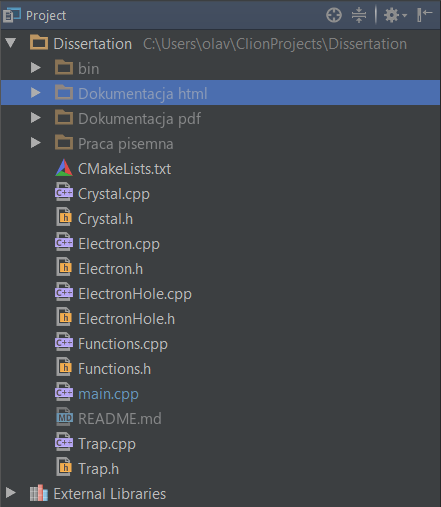
\includegraphics[width=15cm, height=14cm]{strukturaprojektu}
\caption{Struktura projektu.}
\label{fig:Struktura projektu}
\end{figure}

\section{Kod}
\subsection{Konwencja nazw}
W czasie tworzenia projektu kierowano się standardowym, spójnym stylem nazywania klas, metod i zmiennych.
 
Nazwy klas zaczynają się z wielkiej litery. Jeśli nazwa zawiera więcej niż jedno słowo to każde z nich zaczyna się wielką literą np. \textit{ElectronHole}. 

Nazwy zmiennych oraz metod zaczynają się z małej litery. Jeśli nazwy złożone są z wielu słów, każde kolejne słowo - poza pierwszym zaczyna się z wielkiej litery np. \textit{tunnelEffectProbability(double time, double tau)}. 

Argumenty funkcji zaczynają się z małej litery. W przypadku użycia argumentu składającego się z wielu wyrazów oddzielane są one znakiem '\_'  np. \textit{Crystal(long long int n\_el, long long n\_holes, double min, double max)}.

\subsection{Formatowanie i dokumentacja}

W projekcie użyto spójnego stylu "wcinania" kodu za pomocą funkcji \textbf{Reformat Code} programu CLion (skrót Ctrl + Alt + L). Dzięki temu kod stał się dużo bardziej przejrzysty dla programisty.

Każda z klas została umieszczona w osobnych plikach .cpp oraz .h . W plikach .h znajduje się deklaracja klasy wraz z jej metodami i zmiennymi. W plikach .cpp zostały umieszczone implementacje metod dla odpowiednich klas. 

Aby kod był łatwiejszy do zrozumienia oraz dalszego rozwijania wygenerowana została dokumentacja projektu wykonana za pomocą programu \textbf{doxygen}. Zawiera ona informacje na temat metod i składowych wszystkich wykorzystywanych klas. Stworzono dwie wersje dokumentacji: \href{https://github.com/Sharkuu/Dissertation/blob/master/Dokumentacja\%20pdf/Dokumentacja.pdf}{\emph{PDF}} oraz \href{http://dokumentacja.c0.pl/}{\emph{HTML}} (umieszczona na darmowym hostingu cba.pl).

\section{Klasy}
Każda z klas posiada własne metody w zależności od swojego przeznaczenia.

Klasa \textit{Electron} odzwierciedla cząstkę elementarną - elektron. Zmiana ilości tych cząstek w stanie wzbudzonym tj. znajdujących się w pułapce jest głównym celem wykonania tej symulacji.

\textit{ElectronHole} jest reprezentacją dziury elektronowej, z którą to elektron po wykorzystaniu zjawiska tunelowego zrekombinuje. Głównymi składowymi tej klasy są: wektor pozycji dziury, wskaźnik na obiekt typu \textit{Trap} oraz energia dziury wyrażona w elektronowolotach. 

Klasa \textit{Trap} odpowiada defektom w sieci krystalicznej czyli pułapkom, które mogą przechwycić elektron lub dziurę elektronową. Posiada metodę \textit{isOccupied()}, która jest warunkiem sprawdzanym za każdym razem, gdy symulowany jest efekt tunelowy. Na potrzeby wykonania tej symulacji założono, że na samym jej początku wszystkie obiekty reprezentujące elektrony oraz dziury elektronowe znajdują się już w pułapkach. Oznacza to, że konstruktor tej klasy ustawia wskaźnik \textit{electron} na podany obiekt typu \textit{Electron}. Dodatkowo w symulacji ustalono, że dany elektron jeśli spełni warunek wystąpienia zjawiska tunelowego - po jego zajściu i rekombinacji z dziurą - nie może przetunelować ponownie. Zostało to podyktowane zmniejszeniem oczekiwanego czasu działania programu.

Klasa \textit{Crystal} reprezentuje rzeczywisty kryształ, który będzie poddany symulacji zaniku sygnału luminescencyjnego. Zawiera on w sobie inne obiekty takie jak:

\begin{itemize}
\item Elektrony
\item Dziury elektronowe
\item Obiekty odpowiadające defektom sieci krystalicznej - tzw. pułapki
\end{itemize}

Jest to główna klasa zarządzająca całą symulacją. Posiada metody wyliczające niezbędne parametry równania \ref{eq:1}, a także zapisujące wynik działania programu do pliku w odpowiednich jednostkach.





\section{Opis działania programu}



W celu otrzymania danych niezbędnych do wygenerowania wykresu zależności między ilością elektronów w pułapkach a upływem czasu, uruchomiono stworzony program. Obiekt \textit{Crystal} w swoim konstruktorze generuje podaną ilość dziur elektronowych, pułapek oraz elektronów, a następnie przechowuje je w oddzielnych kontenerach. Dla każdej z tych cząstek wywoływany jest konstruktor (ustawiający współrzędne położenia) z argumentami, które są losowane z podanego wcześniej przedziału (wartości są podane w Angstremach tj. 1 Å = $10^{-10}$m. Jednostka ta nie jest jednostką układu SI, lecz jest stosowana w fizyce przy opisywaniu obiektów i zjawisk zachodzących w skali atomowej). Jak podkreślono wcześniej, symulacja zakłada, że na jej starcie każdy elektron znajduje się w pułapce. Powoduje to, że para elektron - pułapka ma identyczne współrzędne położenia, a także obiekt klasy \textit{Trap} przyjmuje wskaźnik na uwięziony w nim elektron.

Następnie za pomocą metody \textit{startSimulation(int time)} obiektu klasy \textit{Crystal} rozpoczyna symulację. Symulowany upływ czasu  zależy od wartości argumentu \textit{time}, który jest wyrażony w dniach tj. wywołanie \emph{startSimulation(365)} oznacza rozpoczęcie działania symulacji symulującej efekt zaniku sygnału luminescencyjnego w czasie 1 roku.

Podczas wykonywania symulacji każda pułapka elektronowa jest sprawdzana, czy przechowuje w sobie uwięziony elektron. Jeśli warunek jest spełniony, to dla elektronu oraz dziur elektronowych znajdujących się w pułapkach, za pomocą wzoru \ref{eq:1} wyliczane jest prawdopodobieństwo zajścia efektu tunelowego. Jeśli prawdopodobieństwo jest mniejsze ( ponieważ wzór \ref{eq:1} oblicza prawdopodobieństwo, że tunelowanie nie zajdzie) od losowej liczny z zakresu [0,1] to elektron opuszcza swoją pułapkę (wskaźnik obiektu klasy \textit{Trap} na elektron ustawiany jest na wartość \textit{NULL}), a następnie zmienia swoje dotychczasowe położenie na współrzędne, do których przetunelował (współrzędne centrum rekombinacyjnego/dziury). Powtarzane jest to tak długo, aż program zasymuluje podany mu wcześniej czas trwania symulacji.  Jak wynika z założeń projektu wspomnianych wcześniej - jeśli elektron przetunelował do centrum rekombinacji przynajmniej raz, nie będzie on brał więcej udziału w obliczaniu prawdopodobieństwa zajścia efektu tunelowego. 

Po skończeniu symulacji, program zapisuje do pliku tekstowego otrzymane wyniki w formacie \textit{czas;ilość elektronów w stanie wzbudzenia}, gdzie czas wyrażony jest w $ \log(\frac{t}{2 dni}) $, a ilość elektronów oznacza jaka część z początkowych elektronów nadal znajduje się w pułapkach. Za pomocą skryptu \textit{wykres.plt}
w folderze \href{https://github.com/Sharkuu/Dissertation/tree/master/bin/Release}{\textit{bin/Release}} generowany jest odpowiedni wykres ilustrujący otrzymane dane. 

Przykładowo wygenerowany wykres (analiza otrzymanych wykresów znajduje się w dalszej części pracy):

\begin{figure}[H]
\centering
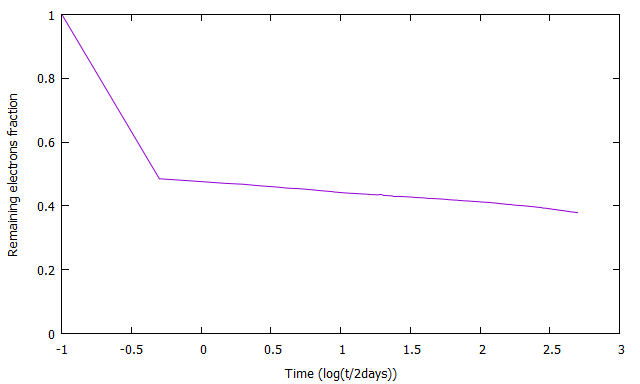
\includegraphics[width=15cm]{wykres1}
\caption{Przykładowa wizualizacja otrzymanych danych}
\label{fig:example}
\end{figure}


\chapter{Analiza wyników}
\chapter{Dalszy rozwój programu}
Projekt posiada podstawową funkcjonalność symulującą atermiczny zanik sygnału luminescencyjnego w skaleniach. Może być rozwinięty i ulepszony o dodatkowe funkcje.

Jak zaobserwowano podczas wykonywania symulacji największą trudnością w działaniu programu jest jego złożoność obliczeniowa, a co za tym idzie czas wykonywania programu. Na chwilę obecną podczas trwania symulacji każdy elektron, który może przetunelować do centrum rekombinacji jest porównywany ze wszystkimi dziurami elektronowymi do czasu spełnienia warunku zajścia efektu tunelowego \ref{eq:1}. Oznacza to, że elektron traktuje każdą dziurę na równi z innymi dziurami. Jak wynika ze wzoru \ref{eq:2} na prawdopodobieństwo zajścia efektu tunelowego w znacznym stopniu wpływa odległość między pułapką z elektronem, a centrum rekombinacji. Dlatego też przy dalszym rozwoju programu należy zoptymalizować kod w taki sposób, aby dziury znajdujące się bliżej elektronu miały wyższy priorytet przy wyliczaniu prawdopodobieństwa tunelowania tzn. były rozważane wcześniej niż dziury odległe. 

Jednym z pomysłów takiej optymalizacji jest użycie drzewa \emph{kd} (w tym przypadku k = 3) czyli podział kryształu skalenia na \emph{N} regiony. Dla każdego elektronu oraz każdej dziury przechowywana byłaby dodatkowa informacja na temat ich przynależności do danego regionu, określana na podstawie współrzędnych cząstki. Gdy dla danego elektronu rozważane byłoby prawdopodobieństwo zajścia efektu tunelowego, do jego wyliczenia w pierwszej kolejności wybierane zostaną dziury uwięzione w tym samym regionie. Jeśli efekt tunelowania nie zaszedł to w zależności od dalszej implementacji program mógłby uznać, że dla tej iteracji elektron nie będzie tunelował lub kontynuowałby sprawdzanie prawdopodobieństwa w sąsiadujących regionach.

Jak zaobserwowano na wykresach w rozdziale \hyperref[wynik:wykres]{4} na początku działania symulacji otrzymano znaczny spadek ilości wzbudzonych elektronów, a dopiero potem wykres kształtem przypomina funkcję liniową. Jest to spowodowane losowym ustalaniem współrzędnych cząstek, przez co przy starcie programu część elektronów znajduje się bardzo blisko dziur umożliwiając zajście efektu tunelowego. Aby ulepszyć otrzymywany wykres, należałoby zaimplementować funkcję, która będzie monitorowała zapisywanie wyników tak, aby pod uwagę brane były tylko dane po początkowym spadku ilości elektronów wynikającym z losowych współrzędnych startowych. Przykładowy wykres wyglądałby wtedy następująco:
\begin{figure}[h]
\centering
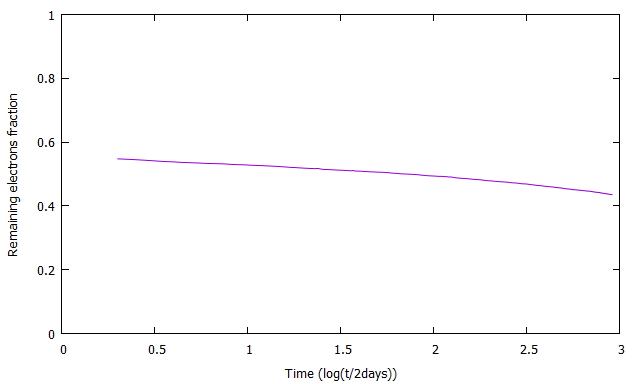
\includegraphics[width=17cm]{przyklad_ulepszony}
\end{figure}

Inną możliwością rozbudowy programu jest dodanie nowej funkcjonalności. Obecnie kroki czasowe przy sprawdzaniu prawdopodobieństwa zajścia tunelowania są równe. Z funkcji prawdopodobieństwa tunelowania wynika, że dobrym pomysłem byłoby wykorzystanie kroków logarytmicznych - na początku działania symulacji używane są małe przedziały czasowe np. sekundy, następnie minuty, potem godziny, dni, lata, dziesiątki lat itd.

Aby program dostarczał bardziej miarodajne dane, należałoby również umożliwić elektronom wielokrotne tunelowanie. W obecnej implementacji elektron po przetunelowaniu nie jest brany pod uwagę w kolejnej iteracji przy wyliczaniu prawdopodobieństwa zajścia tego efektu. W rzeczywistym krysztale zdarza się jednak, że ten sam elektron może tunelować większą ilość razy.

Istnieje również możliwość łatwej zmiany kodu w celu użycia różnych wzorów na prawdopodobieństwo zajścia efektu tunelowego oraz zmiany sposobu rozkładu ładunków podczas tworzenia obiektu kryształu. Obecnie używany jest rozkład jednostajny ciągły, lecz nic nie stoi na przeszkodzie zmiany go na np. rozkład Gaussa. 
\chapter{Wnioski}



\begin{thebibliography}{wstep,technologie}

\bibitem{struktura_pasmowa}
  \emph{Instrukcja do ćwiczenia laboratoryjnego z dozymetrii promieniowania jonizującego dla
studentów specjalności Fizyka Medyczna i pokrewnych}, WFiIS AGH, Kraków 1993, s.3 rys. 1
\bibitem{tunel_pic}
Piotr Psuja,
\emph{Właściwosci luminescencyjne i katodoluminescencyjne
nanometrycznych kompozytów ITO (In2O3/SnO2)
domieszkowanych jonami ziem rzadkich}, Wrocław 2009, s.14 rys. 3.1
\bibitem{wzor}
D.J. Huntley,
\emph{An explanation of the power-law decay of
luminescence}, Styczeń 2006, s.1360 równanie 1

\bibitem{c++}
\url{http://en.cppreference.com/w/cpp}
\bibitem{cpp}
Stephen Prata, \emph{ Język C++. Szkoła programowania. Wydanie V}, Helion, 2006
\bibitem{}
Andrzej Bluszcz, \emph{Datowanie luminescencyjne osadów czwartorzędowych - teoria, ograniczenia, problemy interpretacyjne}, Gliwice 2000
\end{thebibliography}




\end{document}